\documentclass{article}

\usepackage{graphicx}% Include figure files
\usepackage{amsmath,amssymb}% Include figure files
\usepackage{dcolumn}% Align table columns on decimal point
\usepackage{bm}% bold math
\usepackage{caption}
\usepackage{hyperref}
\usepackage{subcaption}
\usepackage{xcolor}
\usepackage[margin=1in]{geometry}

\newcommand{\todo}[1]{ {\color{red}[{\bf TODO:~{#1}}]}}
\let\arrvec=\vec
\renewcommand{\vec}[1]{\mathbf{#1}}

\DeclareMathOperator{\atantwo}{atan2}

\begin{document}

%\preprint{AIP/123-QED}

\title{Classifying Fanaroff-Riley Radio Galaxies}
\author{Josh Marsh}

\maketitle

\section{\label{sec:level1}Introduction}

Recent decades have seen a drastic increase in the amount of data available to astrophysicists. More than ever, efficient and effective data analysis techniques are a critical component much of the research in the field today. With recent advances in deep learning, convolutional neural networks (CNNs) have demonstrated extraordinary success in image classification and have achieved state of-the-art results on various tasks. This makes them well suited for the classification of radio galaxies. Recently, the successful application of these networks have resulted in many discoveries in the field. Notable examples include the search for and the analysis of gravitational lenses. Here we show their successful application to the classification of Fanaroff-Riley radio galaxies. We demonstrate an improvement of (insert number) over previous studies.

\todo{Test on Aniyan}

We consider the classification task of radio galaxies with active nuclei under the Fanaroff-Riley scheme. Under this scheme, galaxies that decrease in luminosity as the distance from the galactic nuclei increases are designated as FR-I, and sources that increase in luminosity towards the outer parts of the nuclei as FR-II. The morphological differences between the two classes in radio images have allowed experts to classify candidates visually with a reasonable degree of accuracy. However, the large pool of potential candidates has limited the confirmed cases to 233 FR-I's (double check) and 123 FR-IIs. The citizen science project Radio Galaxy Zoo has allowed for crowd sourcing the classification task, with (what were the results?). While this has increased the number of examples available to researchers, the sample size is still small enough to make it difficult apply the state of the art image classification methods such as deep learning. Recently, Aniyan and Thorat showed moderate success with convolutional neural networks, achieving a classification accuracy of ## and ## for FR-I and FR-II galaxies, respectively. 

\todo{why is this problem important?}

A core issue with classification tasks in the radio domain is that it is difficult to evaluate the success of classifiers due to the lack of past studies to compare new results to. Up until recently, there was insufficient data to attempt most machine learning techniques. In essence, this means that over twenty years of machine learning methods remain untested on the task, leaving a potential wealth of information undiscovered. In addition, the success of many machine learning algorithms on image classification tasks is based upon performance on optical images - radio imagery.

\todo{different in what way?}

We introduce HOGnet, a tensor-base optimizable feature extractor inspired by the Histogram of Oriented Gradients (HOG) descriptor. Here we show that creating multiple representations of images in the form of localized intensity gradient vectors (how to say this??), we find that HOGnet drastically decreases the time it takes for a model to converge on the optimal weights (say better!) and increases model accuracy. 

\todo{input from Matt on this sentence}

This allows us to successfully train a slightly modified version of the state of the art image classifier VGG19 from scratch on only 62 samples per class. We train HOGnet on our randomly augmented radio images of size 384x384x1 pixels with final dense classification layer and weights manually initialized. We then train our VGG19 model of 2,800,000 parameters on the 48x48x32 outputs of HOGnet to an accuracy 95.5\% accuracy. To demonstrate the extent to which HOGnet reduces problem complexity, we train a vastly simplified version of our HOGnet + VGG19 model of 7,442 parameters to an accuracy of 92.5\%. We use the Adam optimizer and binary cross-entropy. 





\begin{figure}
    \centering
    \begin{subfigure}[b]{0.5\textwidth}
        \centering
        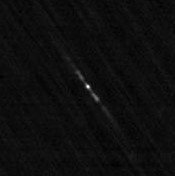
\includegraphics[width=0.7\linewidth]{FR1.jpg} 
        \caption{FR-I}
        \label{fig:subim1}
    \end{subfigure}%
    \begin{subfigure}[b]{0.5\textwidth}
        \centering
        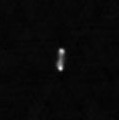
\includegraphics[width=0.7\linewidth]{FR2.jpg}
        \caption{FR-II}
        \label{fig:subim2}
    \end{subfigure}
 
    \caption{Fanaroff-Riley Radio Galaxy Examples}
    \label{fig:image2}
\end{figure}

\subsection{\label{sec:level2}Machine Learning}


Machine Learning is a broadly defined area of computer science and mathematics that allows computer algorithms to develop efficient pattern recognition methods through the iterative process of learning through the experience of performing a task to subsequently increase the performance of the algorithm. For computer vision tasks, this allows large amounts of data to dictate the feature extraction process, removing the need for experts to manually develop tailored solutions - a time-consuming and frustratingly complex endeavor. 

Supervised learning methods, which we employ primarily in this study, aim to identify probability distribution \(p \big(Y |  \vec{x} \big)\) that maps an input vector \(\vec{x} = \big\{x_1, x_2, x_3, ..., x_j\big\}\) to an output value \(Y\). How this is achieved depends on the machine learning method employed. 

\subsubsection{\label{sec:level3}Logistic Regression}

Logistic regression is a simple machine learning model for binary classification. The probability distribution that maps the input feature \(\vec{x}\) to \(Y\), where \(Y \in (0, 1)\), is given by 

\begin{equation}
    y \big( \vec{x} \big) = p \big(z=1 \mid  \vec{x} \big) =  \sigma  \big(\vec{w}^{T}\vec{x}+b \big) 
\end{equation}

where \(\sigma\) is the sigmoid activation function

\begin{equation}
    \sigma  \big(t\big) = \frac{1}{1+e^{-t}}
\end{equation}

The values \(\vec{w}\) and \(b\) are the trainable parameters of our model. Each individual weight \(w_{j}\) in \(\vec{w}\) are scalar values that dictate the extent to which each element \(x_{j}\) of \(\vec{x}\) (for example, the pixel values of an image) affects the probability of input \(\vec{x}\) belonging to either class. Initially set at random, weights are iterativly optimized via the gradient decent until convergence on optimum values. For logistic regression, we optimize via:

\begin{equation}
    \vec{w}_{t+1} = \vec{w}_{t} -  \nabla \delta L \big(\vec{w}_{t}\big) 
\end{equation}

Where \( L\) represents the loss function, \(\nabla \in \big(0, 1 \big)\) is the learning rate, and t is the current time step. The loss function gives the difference between true labels \(Y\) and the model's outputs, i.e how well the model maps \(\vec{x}\) to  \(Y\). For binary classification, we use binary cross-entropy.

\begin{equation}
\nabla L \big(\vec{w}_{t}\big) =  -\frac{1}{N}  \sum_{ \vec{x}, z \in D } \big(z-y \big( \vec{x} \big) \big)\ \vec{x}
\end{equation}

\subsubsection{\label{sec:level3}Neural Networks}

\begin{figure}
\centering
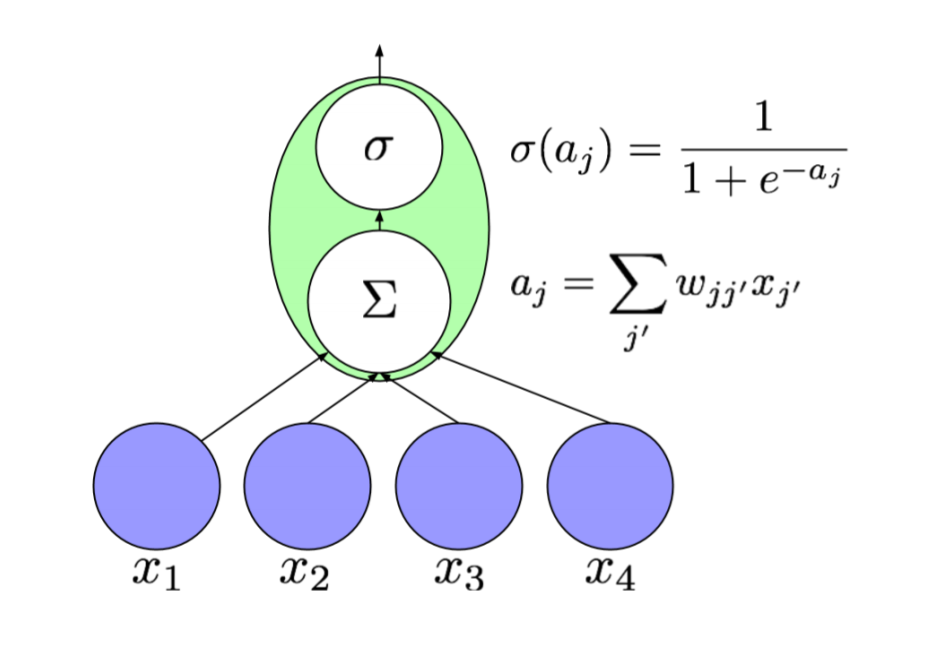
\includegraphics[width=0.5\linewidth]{node.png}
\caption{A single neuron with a sigmoid activation function}
\label{fig:node}
\end{figure}

\begin{figure}
\centering
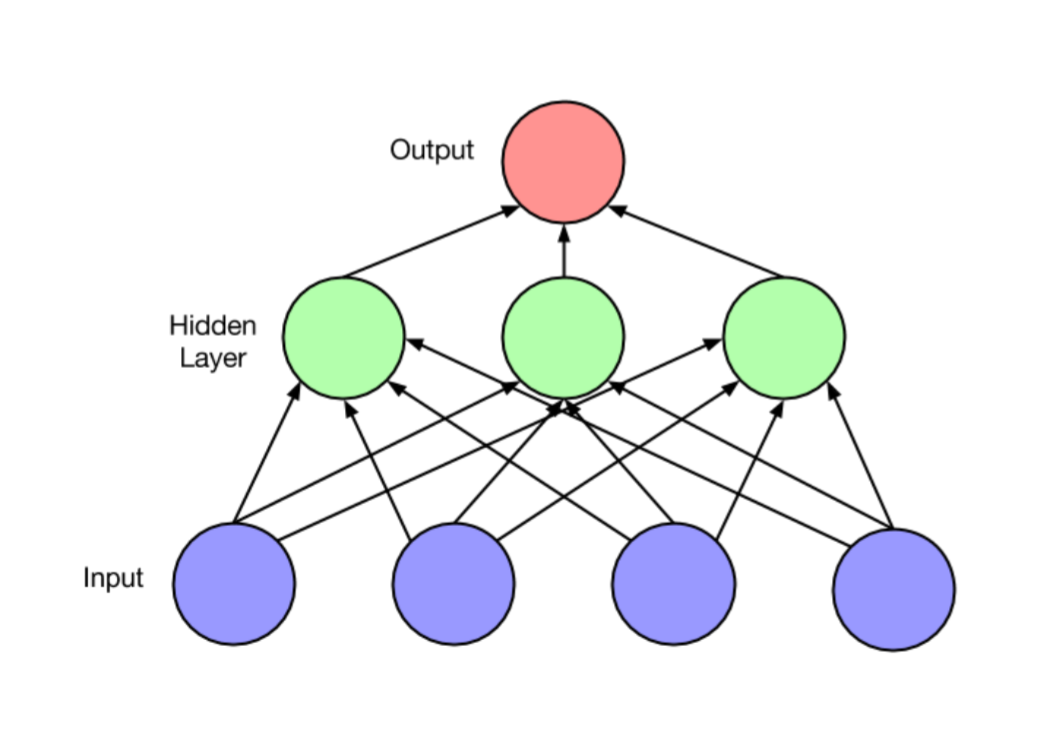
\includegraphics[width=0.5\linewidth]{basic_net.png}
\caption{A Feed-forward Neural Network.}
\label{fig:NN}
\end{figure}

The logistic regression unit, or neuron, shown in figure \ref{node} can be thought of as the fundamental unit of neural networks.  A feed-forward neural network consists of sets of neurons organized into layers, with the output of each layer being the input of the next layer, as shown on figure \ref{NN}. A neuron in a fully connected layer of \(n\) neurons takes the output of each neuron in the preceding layer of \(m\) neurons, giving a total \(n \times m\) connections. More layers can allow networks to identify higher-order complex correlations with fewer parameters (weights) and to be more easily trained. 

In convolutional neural networks, the weights of a layer are organized in multiple two-dimensional matrices called filters. The output array of a convolutional layer is the result of the convolution of each of these filters with the input array (for example, an image). This allows networks to retain two- and three-dimensional structures of input data and to extract the specific patterns that are learned by weight filters. 

\section{\label{sec:level1}Our Approach}
A core problem for quantitatively classifying images is that in many cases no single feature exists that can be used to infer the class of the image. Human classification is a complicated and dynamic process build up through millions of years of evolution. By observing an extremely minimal number of examples, we are able to intuitively infer features of importance to the object's class, subsequently allowing us to determine the class of an object by observing the degree to which each relevant feature is present, and taking a mentally weighted sum to determine which class it is most likely to belong to. It is extremely difficult to define an algorithm that mimics this approach.

Take the FR-I and FR-II classification task. Visually, the radio object's class is often clearly evident. FR-I galaxies frequently possess a few distinct features. These include that the brightest points are always at the center of the radio source and the change in brightness is usually gradual and inversely proportional to the distance from the enter of the source.  FR-II radio galaxies, on the other hand, often comprise of two points that are equidistant and form a strong linear correlation with the source, and are significantly brighter than the actual source itself. We could, in principle, take a single one of these features and build a classifier. Take the gradient for example. If the change in brightness for an FR-I source is, as a general rule, more gradual than that of an FR-II source, we can use this to determine a source's class. To illustrate: by taking the mean magnitude of the gradient for each pixel in a class for half the data, and then classifying the other half of the data based upon which value the mean gradient magnitude for each image is closest to gives an accuracy of 52.1\%. If we are to achieve an accuracy that is remotely within the range of human performance, we need to take into about all relevant features. While the degree to which these features are present in a sample can drastically vary, it is generally possible to classify a sample based upon a dynamic combination features. 

If we were to take this approach algorithmically, that is quantitatively determining the degree to which each of the relevant features exists and taking the weighted sum to determine the probability of the sample belong to either class, we would be performing feature engineering. This is not desirable. While theoretically capable of achieving high accuracy, many of the individual features are extremely difficult to quantify, and are often areas of ongoing research in their own right. In addition, feature engineering is difficult to implement and is highly inflexible, making it hard to adapt to similar tasks. Due to these reasons, we instead take a machine learning based approach. 



\section{\label{sec:level1}HOGNet}

Machine Learning classifiers learn to extract the features directly from an images pixels that are relevant to the images class through the trial and error process of reinforcement learning. While highly effective when enough examples exist to adequately train a model's parameters, when there is not, the results can be sub-optimal. A reason for this is that the patterns that represent image features are not necessarily intuitive in the form of an matrix of pixel intensity values. This makes in the learning these features a computationally exhaustive process. For this reason, we turn the Histogram of Orientated Gradients (HOG) feature extractor, to convert our data into a format makes our classifiers job easier - that is, it keeps information that is relevant to the objects classification and removes information that is not. 

A HOG descriptor extracts an images spatial information in the form of a flattened vector of concatenated histograms that contain the orientations of the pixel intensity gradients for defined portions of the image. We implement HOG as a set of tensor operations.

\subsection{\label{sec:level2}Tensor-based HOG Derivation}


For input \(X \in \mathbb{R}^{l\times w}\), we calculate the gradients \(\Delta\) via convolution with the Prewwit operators \(\rho_x\) and \(\rho_y\), such that 

\[
\rho_x = \begin{bmatrix} 
-1 & 0 & 1 \\
-1 & 0 & 1 \\
-1 & 0 & 1 \\
\end{bmatrix}
\]

\[
\rho_y = \begin{bmatrix} 
{-1} & {-1} & {-1} \\
0 & 0 & 0 \\
1 & 1 & 1 \\
\end{bmatrix}

\]

\[
\Delta 
=
\begin{bmatrix}
    \rho_x \\
    \rho_y
\end{bmatrix}
\circledast
X
\in \mathbb{R}^{h\times w \times 2}
\]

We calculate the gradient orientations \(\theta\) and the magnitudes \(\mu\) via
\[
\theta = \atantwo \big(\Delta_y, \Delta_x \big)
\in \mathbb{R}^{h\times w}
\]

\[
\mu = \lVert \mathbf{\Delta} \rVert_2
\in \mathbb{R}^{h\times w}
\]

To restrict all operations to the tensor domain, we approximate the previously employed histogram bin construction scheme - voting via bi-linear interpolation - as the scalar projection of vectors onto bin unit vectors. Since this is defined as a simple dot product between vectors, we implement this as a Convolution operation, with the angle vectors as the input and the bin unit vectors as the kernels, where each kernel represents a unit vector of shape \(\big(1,  1,  2 \big) \) that operates on each element of the gradient vector array \(\phi\) of shape \(\big(h, w, 2 \big) \). We calculate \(\phi\) via convolution:

\[
\phi = 
\begin{bmatrix}
    \mu \circledast \sin{\theta}\\
    \mu \circledast \cos{\theta}
\end{bmatrix}
\in \mathbb{R}^{h\times w \times 2}
\]


We define \(b\) regions of equal size in range \(\big(-\pi, \pi \big)\), each of which has a center angle \(\theta_i\). For \(i\) in range \(\big(0, b-1 \big)\), we define the center angle \(\theta_i\) as \(\frac{2 \pi}{b}\big(i+ \frac{1}{2} \big)-\pi\). For each \(\theta_i\) we generate a unit vector, giving us \(\Gamma \in \mathbb{R}^{2\times b}\). We calculate the votes each angle gives gives to each bin region \(b\) by convolving \(\phi\) with weight array \(\Gamma\).

\[
V = \Gamma \circledast \phi \in \mathbb{R}^{h\times w \times b}
\]


 A Relu activation function operates on the output to ensure that only positive vector projections count for the voting operation. 
 We separate \(V\) into equal sized cells of shape \(\big(c, c \big)\). For each cell, we sum all votes depth-wise, giving us cell array \(C \in \mathbb{R}^{h_c\times w_c \times b}\) where \( h_c=\frac{h}{c} \text{ and } w_c=\frac{w}{c}\).  
 
 Cells are grouped into overlapping blocks of \(\big(B, B \big)\) cells. The block stride is C pixels, such that each cell is covered by \(B^2\) blocks. We implement the required reshaping operations for block construction as \(B^2\) separate depth-wise convolution operations with zero padding, where for each variation of the kernel of shape \(\big(B, B \big)\) where all elements are equal to zero bar one, a separate operation exists. For \(B=2\), the block construction kernels are:
 
 \[
B_{1, 1} = \begin{bmatrix} 
1 & 0  \\
0 & 0  
\end{bmatrix}
\]

 \[
B_{1, 2} = \begin{bmatrix} 
0 & 1  \\
0 & 0  
\end{bmatrix}
\]
 
  \[
B_{2, 1} = \begin{bmatrix} 
0 & 0  \\
1 & 0  
\end{bmatrix}
\]

\[
B_{2, 2} = \begin{bmatrix} 
0 & 0  \\
0 & 1  
\end{bmatrix}
\]

We concatenate the outputs of each depth-wise convolution layer, giving the un-normalized block array \(\Lambda\).

\[
\Lambda \in \mathbb{R}^{h_c\times w_c \times b \cdot B^2}
\]
 

 We normalize \(\Lambda\) along its last axis:

\[
\Lambda_{i, j, :}
\leftarrow 
\frac{\Lambda_{i, j, :}}{\sqrt{\lVert \mathbf{\Lambda_{i, j, :}} \rVert_2 + \epsilon}}


\]

where \(\epsilon\) is a small positive constant to ensure there are no divisions by zero. \(\Lambda\) is further normalized by:

\[
\Lambda 
\leftarrow 
\frac{\Lambda}{\sqrt{\lVert \mathbf{\Lambda} \rVert_2 + \epsilon}}
\]

and again by:

\[
\Lambda 
\leftarrow 
\frac{\Lambda}{\sqrt{\lVert \mathbf{\Lambda} \rVert_2 + \epsilon}}
\]

The final feature tensor \(\Lambda\) for a single image is an array with both height and width reduced by factor of \(c^2\) and with the channel axis increased by a factor of \(b \times B^2\) - that is, \(b\) feature maps each representing intensity gradients in a defined angle range each represented \(B^2\) in a different local normalization region for each element of block cell \(\big(B, B \big)\). 

\subsection{\label{sec:level2}Implementation Details}

For gradient intensity calculations, we use a single Convolution2D layer with 2 filters of size \(\big(3, 3\big)\), a stride of 1, and zero padding. We initialized the weights as each of the Prewwit operators with added Gaussian noise scaled by \(10^{-2}\) and use no bias. Similarly, for the vote calculation operation we use a Convolution2D operation with \(b\) filters (one for each bin) of size \(\big(1, 1\big)\), a single stride, no bias, and with weights preset as bin unit vectors. A Relu activation function operates on the output to curb the influence of negative projections. To sum all elements in each cell depth-wise, we apply an average pooling operation and then multiply each cell by \(c^2\). For simplicity, we assume the input images have height and width dimensions of equal size that are divisible by \(c \times B\) and have a single colour channel (i.e greyscale). The reshaping required for the block construction operations are broken into separate depth-wise Convolution2D operations with weights preset to the block construction arrays (shown above) followed via a Concatenation along the channels axis. For normalization we use \(\epsilon = 10^{}\)


\section{Methodology} 

Machine Learning techniques have been staggering successful in recent years for images classification. However, many of these algorithms, particularly state of the art methods such as convolutional neural networks, rely on vast amounts of images in order to extract useful features for classification. This makes them unsuited for tasks such as the FR-I/FR-II classification problem, where only 123 and 233 (or something) samples are known for the FR-I and FR-II classes, respectively. It is with this in mind that we built HOGnet, which allows us to to convert the images into a format that allows less computationally exhaustive feature extraction. In addition, we employ a number of other methods to tackle this issue, primarily, by artificially increasing the number of samples. We generate unique samples in real time by a applying a random combination of rotations, horizontal and vertical flips, horizontal and vertical translations, and zooms.  While genuine samples are preferable, this technique has been proven to be effective in the past (find sources).  

\todo{find sources}

\subsection{\label{sec:level2}Data}
We use all FRI sources in the FRICAT catalog and all FRII sources in the FRIICAT catalog. For random radio sources, we use a random subsample of the \(n\) sources in the FIRST catalog on Vizier. We get the coordinates of our FR-I sources via the FRICAT catalog on Vizier and the coordinates of our FR-II sources from FRIICAT from \href{http://go.nasa.gov/2jlAMfN}{NASA}. To get the coordinates for the individual components of each the source, we use Vizier to query the region within a 2.35 arcmin radius around the FR-I sources and a 2.68 arcmin radius around the FR-II sources. We pick these radii by taking the minimum gradient of the components per source over a 15 arcsec moving average. We use these coordinates to download images with a width of 10 arcmins from the FIRST cutout server \href{https://third.ucllnl.org/cgi-bin/firstcutout}{here}. To ensure no faulty image are included in the experimental data, we discard any images that contain Nans or have means of 0.

\todo{How do we get Aniyan?}

\subsection{\label{sec:level2}Architectures}
Our two primary models in this report use the same variation of HOGNet as the upper component of their architecture - the bottom component that takes the output of HOGNet as its input being varied and each with its own merits and drawbacks. Based on past research and extensive experimentation, we choose the following HOGNet hyperparameters: 8 bins, cells of size \( \big(8,  8 \big)\), and blocks of size \( \big(2,  2 \big)\). 

\subsubsection{\label{sec:level3}HOGNet-lite}
Optimized for minimal for trainable parameters, HOGNet-lite is by far the smaller of the two variations.
Stacked below HOGNet, the model is made up of two similar convolution blocks followed by a final fully-connected classification block. The convolution blocks each have three Conv2d layers with \( \big(3,  3\big)\) filters of a single stride with same padding, followed by a \( \big(2, 2\big)\) MaxPooling2D Layer. We use 4 filters per Conv2d layer in the first block and  8 in the second. The classification block is comprised of 3 fully connected Dense layers, each with 50 neurons and 0.2 dropouts. These are followed by a final single neuron Dense layer with a sigmoid activation function. All other Dense and Conv2D layers use Relu activations. The model has a total of 7,842 trainable parameters.   

\todo{Check the number of trainable parameters}

\subsubsection{\label{sec:level3}HOGNet-VGG}
Inspired by VGG-19 and modified for this specific task, HOGNet-VGG is our highest performing model by validation accuracy. However, with a total of 1,800,000 trainable parameters, training time is significantly longer. After the top HOGNet component, the model is made up of the first three convolution blocks of VGG-19 with Relu activations. For the classification block, we use 2 Dense layers of 50 neurons with Relu activations and added 0.2 dropouts. This is followed by a final Dense layer with a single neuron with a sigmoid activation function.

\todo{Check the number of trainable parameters}

\subsection{\label{sec:level2}Training}

With the ImageDataGenerator function in Keras, we apply a combination of random rotations up to 180 degrees in both directions, horizontal and vertical flips, and re-sizing by up to 20\%. We generate these continuously from the original images during the training process. As a result, our models never see the same sample twice. For legacy machine learning models, many of which cannot be trained by mini-batches, we generate the data in advance, increasing the number of samples by a factor of 100.  To each augmented image, we add the magnitude of a Gaussian noise scaled down by \(10**10\)  to each image. This is necessary to avoid a vanishing gradient when sections of images had pixel magnitudes of zero due to formatting errors, resulting in gradients of zero that broke the arctan2 function in our tensorflow layer. To fit model assumptions, we re-size all our images to 256 along both axes with Scikit-image and normalize the intensity values of each image individually to \(\big[0, 1\big]\).  Images are randomly shuffled before augmentations are applied, and, if generated in advance, again after augmentations. 

Due to the small dataset combined with the problem complexity, models fail to converge on optimal weights and do not achieve better than random accuracy when a model reaches a critical number of train parameters. \todo{I forget what this is. Need to rerun a lot of tests} While less complex models are able to train, their accuracies are not very impressive. \todo{Think of a better way to say this} To overcome this, we employ a multistage training approach. First, we freeze all weights in the convolution blocks and train the weights in classification block. We also allow all weights in HOGNet that we preset to train. We then unfreeze \( gap\) number trainable layers and allow them to train, repeating this iteratively from the top down of the layers in the convolutional blocks, training until there is no improvement in the loss for 10 epochs or for a maximum of 100 epochs for each stage. 

For all experiments we spit our data into \(\frac{2}{3}\) training and \(\frac{1}{3}\) testing sets along each class, respectively, giving us two equally class imbalanced sets. To avoid class bias in our classifiers, we compute and train on balanced class weights for each of our models. 

We train our models on binary cross-entropy with the Adam optimizer with Adam parameters of \(\beta_1 = 0.9\) and \(\beta_2 = 0.999\) with a learning rate of \(0.001\). Learning rate is reduced if there no drop in loss for 5 epochs.



\section{Results}

\subsection{\label{sec:level2}FR-I vs FR-II}


\subsection{\label{sec:level2}FR vs Random}


\subsection{\label{sec:level2}Aniyan Vs Random}


\subsection{\label{sec:level2}Design Plots}

\begin{figure}
\centering
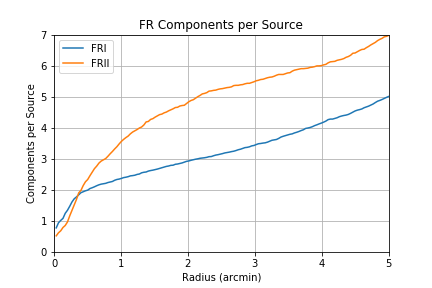
\includegraphics[width=0.5\linewidth]{component_per_source.png}
\caption{Components per FR-I and FR-II source vs Radius around the object in arc minutes}
\label{fig:node}
\end{figure}


\begin{figure}
    \centering
    \begin{subfigure}[b]{0.5\textwidth}
        \centering
        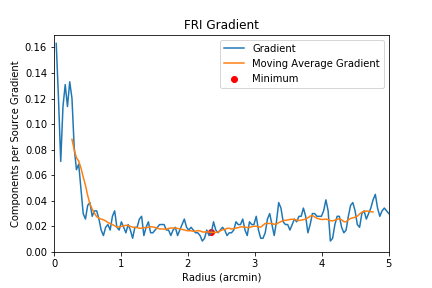
\includegraphics[width=1\linewidth]{fri_grad.png} 
        \caption{}
        \label{fig:subim1}
    \end{subfigure}%
    \begin{subfigure}[b]{0.5\textwidth}
        \centering
        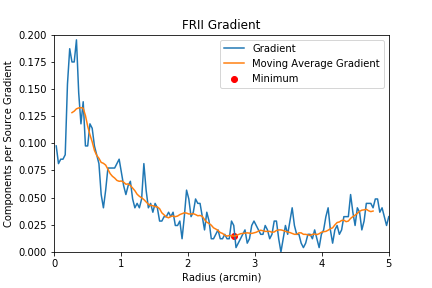
\includegraphics[width=1\linewidth]{frii_grad.png}
        \caption{}
        \label{fig:subim2}
    \end{subfigure}
 
    \caption{Gradient of Components per Source with moving average over a 15 arc second window for FR-I and FR-II}
    \label{fig:image2}
\end{figure}




Results - lots of tables and graphs




\section{Discussion}

The primary benefit of HOGNet is that it allows us to utilize extremely large state convolutional neural networks like VGG19 on an extremely small set of data (HOGNet-lite is a vastly simpler version of HOGNet-VGG, which is heavily inspired by VGG19). HOGNet simultaneously reduces the dimensionality of the vertical and horizontal axes (by \(8\) each in our tests) and while drastically increasing the dimensionality on the third axis (by a factor of 32 in our tests, with \(8\) bins and a block area of \(2^2\)) by way of unique feature maps. Each of these feature maps, representing intensity gradients in varying angle ranges in a different normalization region for each block, can be thought of as the output of a different filter from a Cov2D layer followed by a max-pooling layer - or more accurately, an average-pooling layer. This reduced dimensionality of the first two axes means that, upon passing through successive max-pooling operations, the flattened output tensor of the final convolution block is reduced to \todo{get value} values for HOGNet-lite and \todo{get value} values for HOGNet-VGG, drastically reducing the number of weights in the Dense classification block and thus the overall model complexity.  
    
All models we tested (which granted was not very many) trained up 5-50 times faster on the output array of HOGNet than raw images. As models of higher complexity were unable to converge on a solution and achieve an accuracy higher than random chance, it was not possible to evaluate this for many of the models we tested. Our explanation for phenomena is that HOGNet drastically reduces problem complexity, and thus the time it takes for the optimizer to converge on the weights. It also slightly increased accuracy for all models tested - for logistic regression, by 1\%. As HOGNet enables backpropagation through HOG, we are able to train our initial preset weights boosting accuracy by roughly 2\% with logistic regression.


\section{Code and Implementation}
 
All data preparation, configuration, and management, is handled entirely within python 3.5, relying on the packages Numpy for array manipulation, Scipy for for HOG, and Skimage for it's implementations of legacy machine learning methods, such as Naïve Bayes, Random Forrest Trees, and Support Vector Machines. Neural Netowrks and Logistic Regressions were constructed using Keras, a high-level deep learning library for large scale machine learning, with Google's Tensorflow as a backend. We construct layers in Tensorflow when necessary. Code along with a fully functioning API can be found on Github \href{https://github.com/MatthewJA/thursday}{here} 

\end{document}
%
% ****** End of file aipsamp.tex ******

